%----------------------------------------------------%
%               PROCESAMIENTO DE DATOS               %
%----------------------------------------------------%

\pagestyle{fancy}

\chapter{Procesamiento y Resultados}
\label{procesamiento_datos}

En el presente capítulo, el penúltimo del documento, se analiza el código implementado para materializar las consultas especificadas en el apartado \ref*{definicion_consultas}. A su vez, se publican los resultados obtenidos mediante la ejecución de dichas consultas y a la postre, se detallan las diferencias existentes entre ambos entornos en cuanto a tiempo de ejecución se refiere.

\section{Procesamiento de datos}

El código ejecutado para procesar los datos almacenados en ambos entornos es diametralmente opuesto.\\

Por un lado, en el entorno centralizado, se hace uso de SQL, un lenguaje de consultas totalmente estandarizado desde hace décadas. Ofrece la posibilidad de recuperar cualquier subconjunto de datos utilizando una sintaxis relativamente sencilla.\\

Por el otro, en el entorno distribuido, el proceso se complica de sobremanera ya que es necesario lidiar con varias tecnologías a la vez y tener en cuenta las restricciones que cada una de ellas presenta. Ello implica la conveniencia de utilizar una capa de abstracción superior que unifique el funcionamiento de ambas tecnologías, como por ejemplo un conector, el cual dificulta conocer a ciencia cierta lo que se acaba ejecutando en las capas inferiores.\\

\subsection{Entorno centralizado}

Las consultas SQL lanzadas contra el entorno centralizado no atesoran intríngulis alguna, por lo que se ha optado por omitir los detalle referentes a su sintaxis y presentarlas directamente:\\
 
\subsubsection[]{MYSQL01}

\begin{figure}[h]
	\centering
	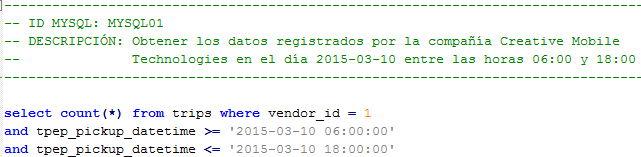
\includegraphics[width=0.9\textwidth]{Ilustraciones/MYSQL01.png}
	\caption{Código referente a la consulta MYSQL01}
\end{figure}

\subsubsection[]{MYSQL02}

\begin{figure}[h]
	\centering
	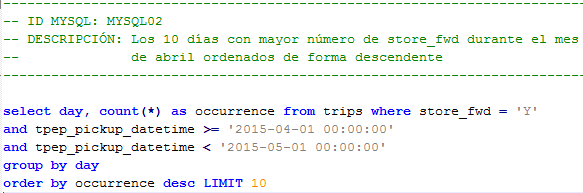
\includegraphics[width=0.9\textwidth]{Ilustraciones/MYSQL02.png}
	\caption{Código referente a la consulta MYSQL02}
\end{figure}

\clearpage

\subsubsection[]{MYSQL03}

\begin{figure}[h]
	\centering
	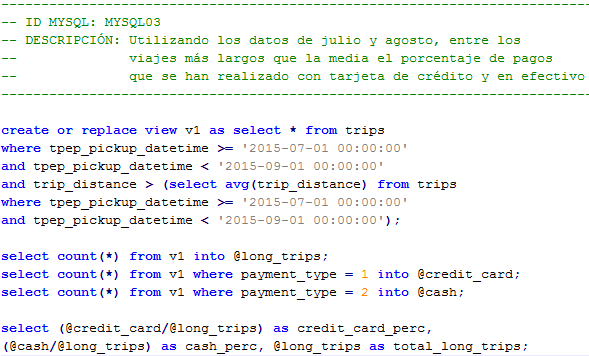
\includegraphics[width=0.9\textwidth]{Ilustraciones/MYSQL03.png}
	\caption{Código referente a la consulta MYSQL03}
\end{figure}

\subsubsection[]{MYSQL04}

\begin{figure}[h]
	\centering
	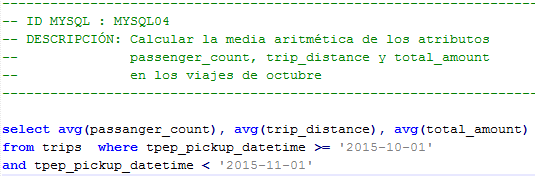
\includegraphics[width=0.9\textwidth]{Ilustraciones/MYSQL04.png}
	\caption{Código referente a la consulta MYSQL04}
\end{figure}

\clearpage

\subsection{Entorno distribuido}

El cuanto al código Java utilizado para representar las consultas del entorno distribuido se refiere, la semántica de su sintaxis ayuda a arrojar luz sobre el uso de cada tecnología, las limitaciones que presentan y la forma en la que se compenetran entre ellas para superar diversas limitaciones.\\

Por todo ello, al contrario que en el apartado anterior, además de ilustrar el código ejecutado, se ha considerado interesante dedicar unas palabras para explicar el rol que adopta cada tecnología dentro de cada consulta.\\

\subsubsection[]{CLU01}

Ejemplo canónico de una consulta contra Cassandra. Se especifican las \textit{Partition Key} 'vendor\_id' y 'dia' para identificar una partición concreta de la tabla y se filtra el contenido de la misma mediante las fechas del \textit{Clustering Column} 'tpep\_pickup\_datetime'.\\

\begin{figure}[h]
	\centering
	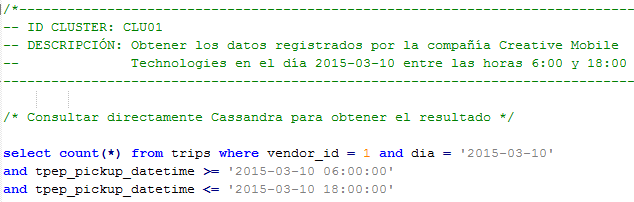
\includegraphics[width=0.9\textwidth]{Ilustraciones/CLU01.png}
	\caption{Código referente a la consulta CLU01}
\end{figure}

\clearpage

\subsubsection[]{CLU02}

El código que se presenta a continuación trata de exponer un caso en el que Cassandra por si sola no es capaz de satisfacer los requerimientos de una consulta y necesita la ayuda de Spark para conseguir el objetivo.\\

Debido a que el atributo 'store\_fwd' no forma parte de la \textit{Partition Key} definida para la tabla, es totalmente imposible realizar una consulta que filtre los datos mediante dicho criterio. La solución del problema pasa por utilizar Spark, ya que permite almacenar en memoria los registros requeridos y computar las operaciones deseadas libre de toda limitación estructural.\\

Con el objetivo de no saturar la memoria, se recomienda encarecidamente cargar desde el sistema de almacenamiento solamente el subconjunto de datos que se desea computar. En este caso particular, se quieren obtener los datos de varias compañías a lo largo de diversos días, lo cual implica lanzar una consulta por cada partición de Cassandra y posteriormente parelelizar cada una de las respuestas para que Spark pueda realizar las operaciones pertinentes.\\    

Para simplificar procesos engorrosos como el recientemente descrito, existe la opción de utilizar conectores gratuitos que posibilitan entrelazar el funcionamiento de ambas tecnologías. Tal y como se puede observar en la figura \ref{fig:consulta_clu02} de la página \pageref{fig:consulta_clu02}, gracias al conector Spark/Cassandra de DataStax\footnote{\url{https://github.com/datastax/spark-cassandra-connector}} basta con crear una lista que contenga tantos objetos como \textit{Partition Key} a consultar y utilizar dicha lista para llamar al método \textit{joinWithCassandraTable}. Este último se encarga de devolver los datos requeridos y cargarlos en memoria de forma totalmente transparente para el usuario.\\

\begin{figure}[h]
	\centering
	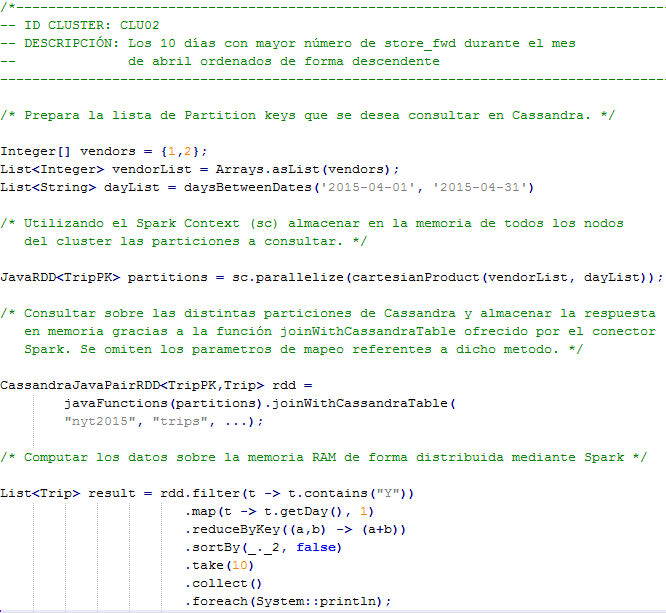
\includegraphics[width=1\textwidth]{Ilustraciones/CLU02.png}
	\caption{Código refente a la consulta CLU02}
	\label{fig:consulta_clu02}
\end{figure}

\clearpage

\subsubsection[]{CLU03}

La mejor forma de optimizar el procesamiento utilizando Spark es iterar sobre una RDD anteriormente cargada en memoria, ya que esta tecnología es capaz de realizar cómputos resilientes sin tener que almacenar los resultados intermedios en disco.\\

Por defecto, Spark sólo almacena información en la memoria durante el cómputo, pero ofrece la posibilidad de \textit{cachear} un conjunto de RDDs para no tener que repetir todas las transformaciones realizadas hasta obtener dicho subconjunto de datos. En la figura \ref{fig:consulta_clu03} de la página \pageref{fig:consulta_clu03} se puede observar cómo la lista \textit{longTrip} es cacheada para a continuación aplicar tres acciones diferentes sobre ella.\\

\begin{figure}[h]
	\centering
	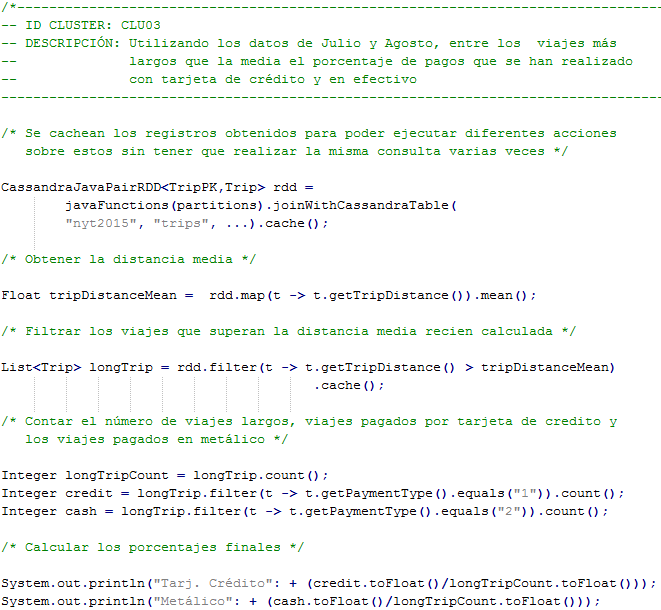
\includegraphics[width=0.9\textwidth]{Ilustraciones/CLU03.png}
	\caption{Código refente a la consulta CLU03}
	\label{fig:consulta_clu03}
\end{figure}

\clearpage

\subsubsection[]{CLU04}

Consulta que imita de forma muy simplificada el proceso Cálculo de Indicadores de Ipanel. No aporta nada novedoso en cuanto a las tecnologías se refiere
pero refleja la praxis recomendada a la hora de realizar agregaciones: calcular las medias de cada día y almacenarlos en una tabla distinta para más tarde utilizar dichos resultados para calcular los informes semanales, mensuales y anuales.\\

\begin{figure}[h]
	\centering
	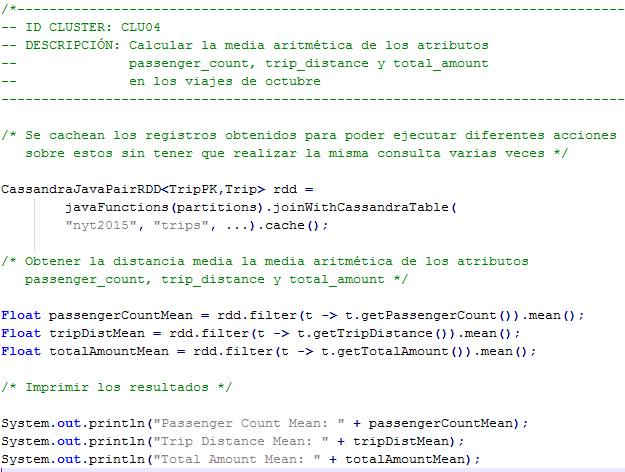
\includegraphics[width=0.9\textwidth]{Ilustraciones/CLU04.png}
	\caption{Código refente a la consulta CLU04}
\end{figure}

\clearpage

\section{Resultados}

Una vez habiendo aclarado los entresijos de cada consulta, es hora de poner el broche final al capítulo presentando los resultados obtenidos a consecuencia de su ejecución.\\

Para realizar dichas consultas ha sido totalmente necesario poblar las bases de datos con anterioridad. Aprovechando esta circunstancia se ha medido el ratio de inserciones por mes ofrecido tanto por MySQL Server como por Cassandra.

\subsection{Inserciones}

Al contrario de lo que se podría esperar inicialmente\cite{rabl2012solving}, MySQL Server ofrece un ratio de escritura 15 veces superior al de Cassandra cuando ambas bases de datos se encuentran vacías. No obstante, su rendimiento decae de forma exponencial a medida que se insertan más registros, llegando a rendir peor que Cassandra una vez habiendo insertado la mitad del dataset. Cassandra, por su parte, demuestra ser capaz de mantener un ritmo de inserción constante en todo momento.\\
 
\begin{figure}[h]
	\centering
	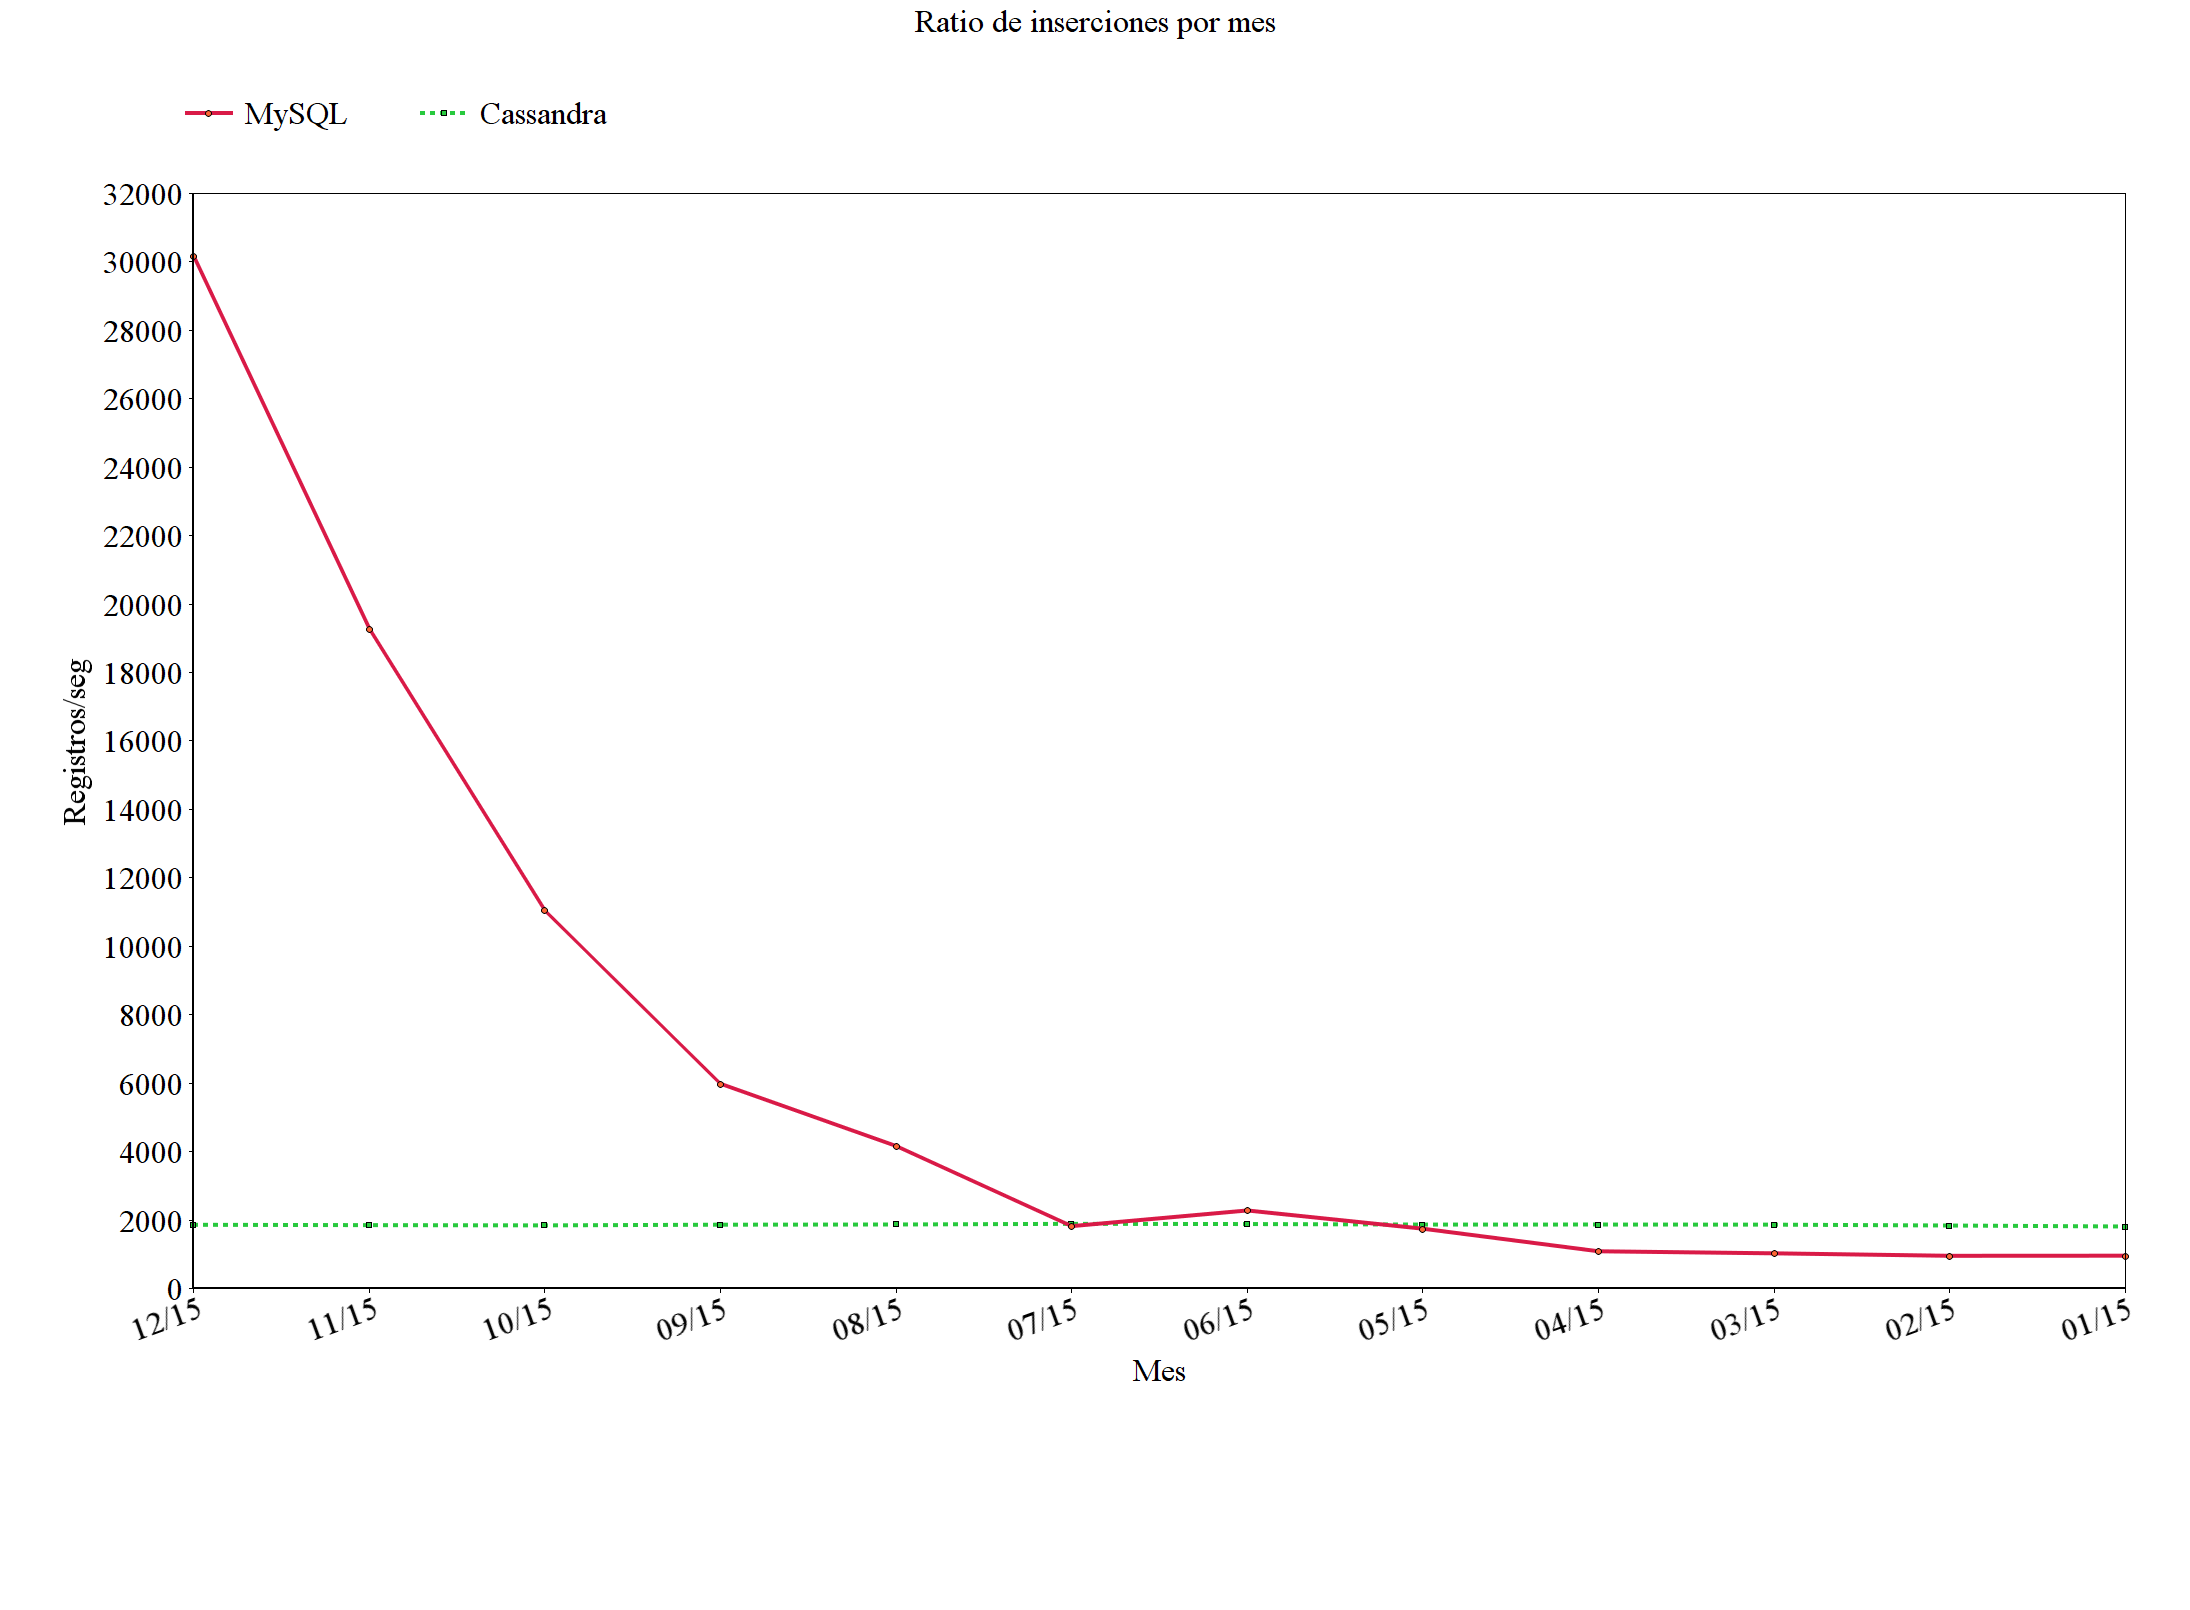
\includegraphics[width=1\textwidth]{Ilustraciones/registrosPorSeg.png}
	\caption{Comparativa tiempos de inserción}
\end{figure}

La causa principal de estos resultados tan inesperados se pueden resumir en los siguientes tres puntos:

\begin{itemize}
	
	\item \textbf{Los nodos comparten disco}: Los nodos virtuales que conforman el clúster hacen uso del mismo disco físico, el perteneciente al ordenador de sobremesa. Ello desemboca en un exceso de operaciones entrada/salida que ralentiza las escrituras. La solución pasa por equipar un disco propio a cada nodo de la infraestructura.
	
	\item \textbf{Las SSTable y el Commitlog comparten disco}: Es posible obtener una mejora aún mayor   separando las escrituras de los Commitlog y las SSTable en discos diferentes. Debido a que el acceso a disco en cada caso es totalmente distinto; mientras que los Commitlog se acceden de forma secuencial, las SSTable no siguen un patrón predefinido, tener los dos directorios en el mismo disco puede hacer que las operaciones del cliente se bloqueen entre ellas. 
	
	\item \textbf{Deficiencias del comando copy}: Cassandra ofrece la opción de cargar los datos almacenados en un fichero CSV mediante el comando \textit{copy}\footnote{\url{http://docs.datastax.com/en/cql/3.1/cql/cql_reference/copy_r.html}}. Al contrario que su homologo \textit{load file}\footnote{\url{https://dev.mysql.com/doc/refman/5.7/en/load-data.html}} de MySQL, el comando \textit{copy} se encuentra diseñado para cargar un número de registros limitados, por lo que su rendimiento decae drásticamente al cargar conjuntos de datos que superen unos pocos miles de registros.
	
\end{itemize}

Aplicando las optimizaciones recientemente expuestas Cassandra sería netamente superior a MySQL en cuanto al ratio de inserciones/segundo se refiere, pero debido a las características de la máquina física utilizada en el proyecto ha sido totalmente imposible exprimir todo el potencial de esta base de datos distribuida.
 
\subsection{Consultas de Lectura}
 
 Con el objetivo de medir el rendimiento de cada entorno, las consultas predefinidas en el apartado \ref{definicion_consultas} de la página \pageref{definicion_consultas} han sido ejecutadas 5 veces cada una. En las figuras \ref{fig:consulta_resumen_mysql} y \ref{fig:consulta_resumen_cluster} se
 recoge el tiempo transcurrido en el procesamiento de dichas consultas, acompañadas por varios indicadores estadísticos que ofrecen un valor añadido a la información presentada.
 
 \begin{figure}[h]
 	\centering
 	\includegraphics[width=1\textwidth]{Ilustraciones/MYSQLTiempos.png}
 	\caption{Resumen de las consultas del entorno centralizado}
 	\label{fig:consulta_resumen_mysql}
 \end{figure}
 
 \begin{figure}[h]
 	\centering
 	\includegraphics[width=1\textwidth]{Ilustraciones/CLUTiempos.png}
 	\caption{Resumen de las consultas del entorno distribuido}
 	\label{fig:consulta_resumen_cluster}
 \end{figure}
 
 \clearpage
 
 Tal y como se ha podido comprobar, la desviación estándar es inferior al 10\% en todos los casos, lo cual implica que la diferencia entre los tiempos obtenidos es muy pequeña, legitimando así  el valor de las medias calculadas.\\
 
 En la figura \ref{fig:consulta_resumen_general} de la página \pageref{fig:consulta_resumen_general} se vislumbra de forma gráfica la inmensa mejora obtenida mediante el entorno distribuido en cuanto a tiempo de ejecución se refiere.\\
 
 En el peor de los casos el ahorro de tiempo es superior al 95\%, 20 o más veces rápido que su consulta homóloga en el entorno centralizado, dejando en clara evidencia la mejora que ofrece el uso conjunto de Cassandra y Spark a la hora de computar volúmenes masivos de datos.\\
 
 \begin{figure}[h]
 	\centering
 	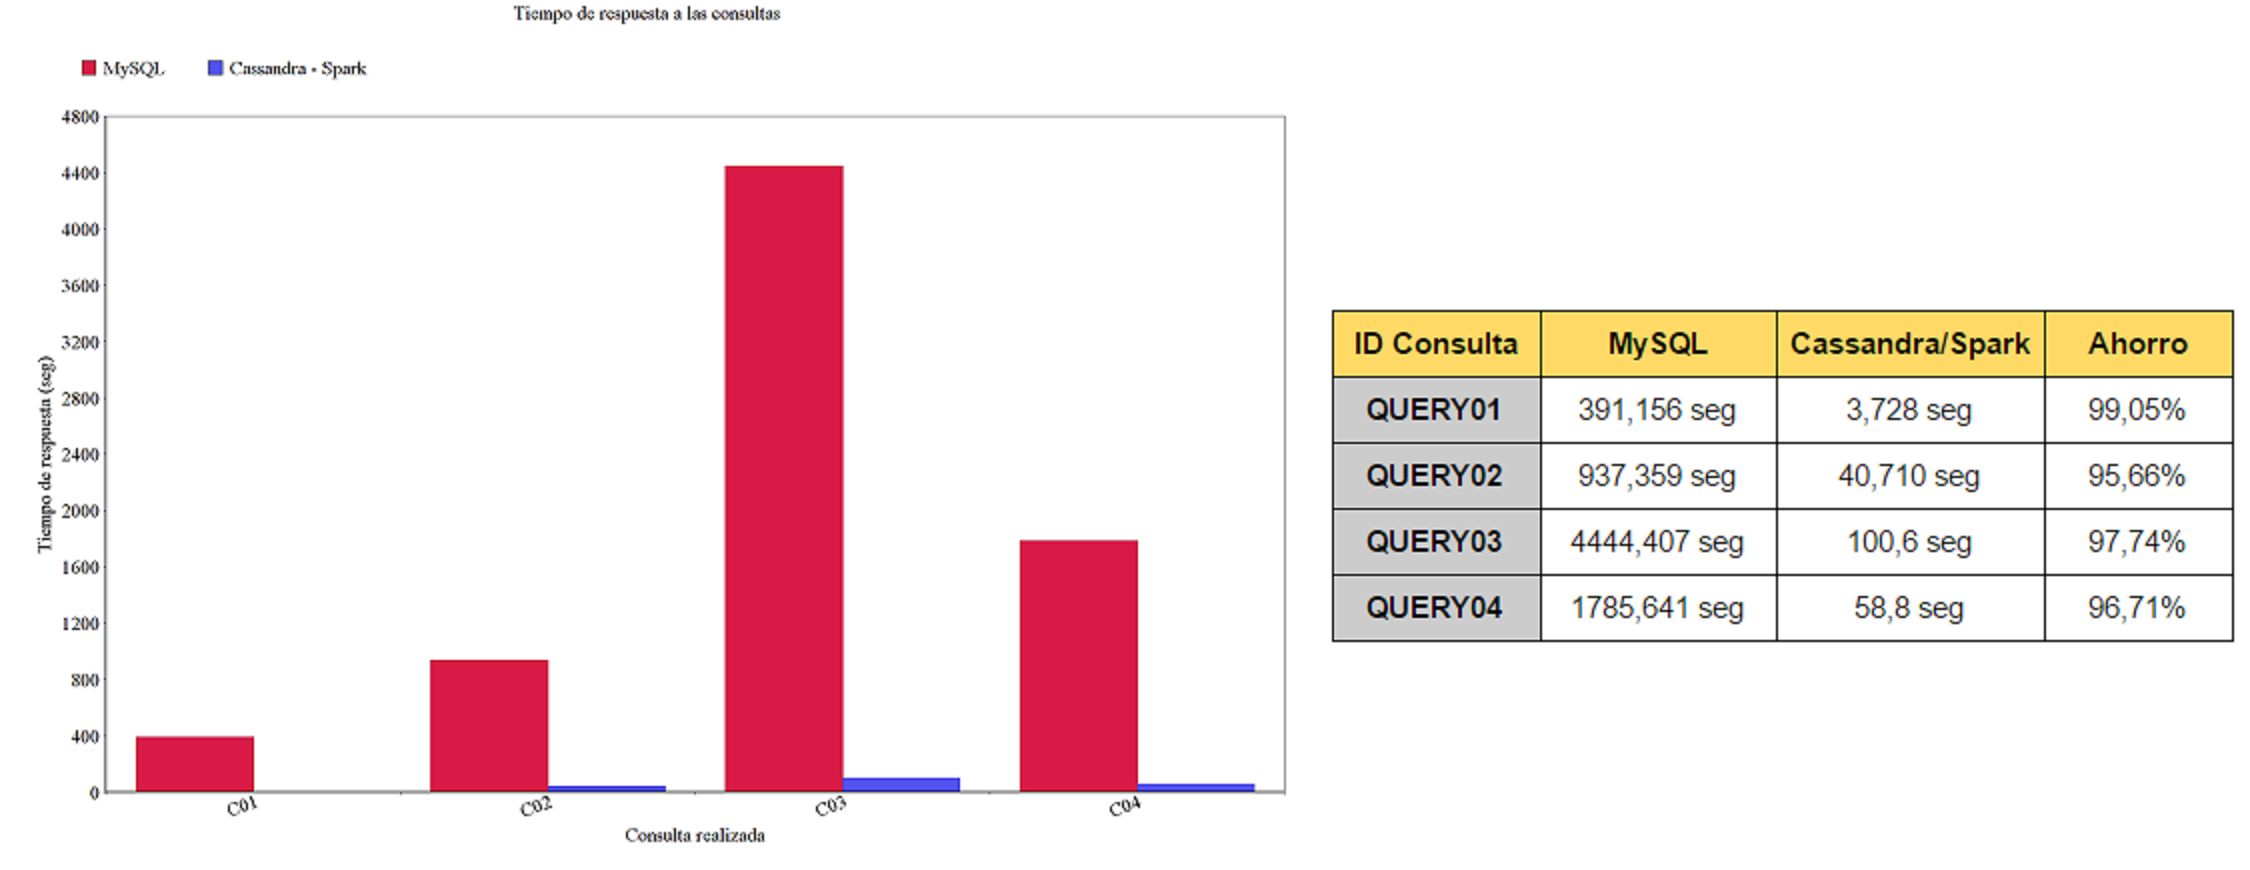
\includegraphics[width=1\textwidth]{Ilustraciones/TiempoRespuestaConsultas.png}
 	\caption{Comparativa entre los resultados de ambos entornos}
 	\label{fig:consulta_resumen_general}
 \end{figure}
 
 
 
 


